\documentclass[slidestop,compress,mathserif]{beamer}
%\documentclass[slidestop,compress,mathserif,handout]{beamer}

%\documentclass[xcolor=dvipsnames,handout]{beamer}
%\documentclass[xcolor=dvipsnames]{beamer}

%\documentclass[handout]{beamer}

%%% To get rid of solutions on handouts:
\newcommand{\soln}[1]{\textit{\textcolor{darkGray}{#1}}}				% For slides
%\newcommand{\soln}[1]{ }	% For handouts

% to get pausing to work properly on slides
\newcommand{\hide}[1]{#1}	% For slides
%\newcommand{\hide}[1]{ }	% For handouts

%\newtheorem{defn}{Definition}

%\usepackage{multicol}
\usepackage{amsfonts}
%\usepackage[pdftex,dvipsnames]{color}
\usepackage{graphicx}
\usepackage{subfigure}
%\usepackage{picinpar}
\usepackage{pifont}
\usepackage{pgf,pgfarrows,pgfnodes}
%\usepackage{wasysym,manfnt,phaistos,empheq}
\usepackage[english]{babel}
\usepackage{pgfpages}
\usepackage{natbib}
\usepackage{hyperref}
\usepackage{multimedia}
%\usepackage{amsfonts,amstext,amssymb,amsbsy,amsopn,amsthm,eucal,latexsym,mathrsfs}
\usepackage{amsmath,amsfonts,amstext,amssymb,amsbsy,amsopn,amsthm,eucal,latexsym,mathrsfs}
\usepackage{ulem}
\usepackage{setspace}
\usepackage{array}
%\usepackage{rotating}
\usepackage{multirow}
\usepackage{verbatim}
\usepackage{multicol}

\setbeamertemplate{navigation symbols}{}

%\usepackage{tikz}
%\usetikzlibrary{arrows,shapes,trees,backgrounds}


%\setbeameroption{show notes on second screen}
%\setbeameroption{show notes}
%\setbeameroption{show only notes}

\definecolor{links}{HTML}{2A1B81}
\hypersetup{colorlinks,linkcolor=,urlcolor=links}

\newtheorem*{principle}{Inscrutibility Principle}
\newtheorem*{punchline}{Punch Line}
\newtheorem{defn}{Definition}

\definecolor{Scarlet}{RGB}{140,17,17}
\definecolor{VassarRed}{RGB}{128,0,0}

% "dinglist" environment
  \renewenvironment{dinglist}[2][blue]
  {\begin{list}{\textcolor{blue}{\ding{#2}}}{}}{\end{list}}
  % Symbol definitions for these lists
  \newcommand{\DingListSymbolA}{43}
  \newcommand{\DingListSymbolB}{243}
  \newcommand{\DingListSymbolC}{224}
  \newcommand{\DingListSymbolD}{219}
  \newcommand{\DingListSymbolCheck}{52}
  \newcommand{\DingListSymbolCross}{56}


  \newenvironment{ballotenv}
{\only{%
\setbeamertemplate{itemize item}{\ding{45}}%
\setbeamertemplate{itemize subitem}{\ding{46}}%
\setbeamertemplate{itemize subsubitem}{\ding{46}}}} {}
\setbeamertemplate{itemize item}{\ding{49}}
\setbeamertemplate{itemize subitem}{\ding{47}}
\setbeamertemplate{itemize subsubitem}{\ding{47}}


%User defined colors: See colors section
\xdefinecolor{oiBlue}{rgb}{0.15, 0.35, 0.55}
\xdefinecolor{gray}{rgb}{0.5, 0.5, 0.5}
\xdefinecolor{darkGray}{rgb}{0.3, 0.3, 0.3}
\xdefinecolor{darkerGray}{rgb}{0.2, 0.2, 0.2}
\xdefinecolor{rubineRed}{rgb}{0.89,0,0.30}
\xdefinecolor{linkCol}{rgb}{0.11,0.49,0.95}	
\xdefinecolor{irishGreen}{rgb}{0,0.60,0}	
\xdefinecolor{darkturquoise}{rgb}{0.44, 0.58, 0.86}
\definecolor{lightGreen}{rgb}{0.533,0.765,0.42}
\xdefinecolor{Regalia}{HTML}{522D80}
\xdefinecolor{ClemsonOrange}{HTML}{EA6A20}

\definecolor{duke@LightGrey}{RGB}{200,200,200}\definecolor{DarkGreen}{RGB}{0,100,0}
\definecolor{Oranges}{RGB}{255,127,0}
\definecolor{LightGray}{RGB}{211,211,211}

%\setbeamertemplate{footline}{%
%  \raisebox{5pt}{\makebox[\paperwidth]{\hfill\makebox[10pt]{\scriptsize\insertframenumber}}}}

\setbeamercolor{equation background}{fg=black,bg=duke@LightGrey}
  % Boxed equation
  \newcommand{\eqbox}[2][0.6]{%
  \centerline{
  \begin{beamerboxesrounded}[lower=equation background,width=#1\hsize,shadow=true]{}
\parbox{#1\hsize}{%
      \[
        \textcolor{black} {#2}
      \]}
  \end{beamerboxesrounded}
}}

\AtBeginSection[] {
  \begin{frame}<beamer>\frametitle{Outline}
    \tableofcontents[currentsection,hideothersubsections]
  \end{frame}
}
%
%
%\AtBeginSubsection[] {
%  \begin{frame}<beamer>\frametitle{Outline}
%    \tableofcontents%[currentsection,currentsubsection]
%  \end{frame}
%}

%\usecolortheme[RGB={82,45,128}]{structure}
%\usecolortheme[RGB={162,80,22}]{structure}
\usecolortheme[RGB={128,0,0}]{structure}
\usetheme[secheader]{Boadilla}
%\usetheme[height=7mm]{Rochester}
%\usetheme{Copenhagen}
%\usetheme{Antibes}
%\usecolortheme{seahorse}
%\usecolortheme{crane}
%\usecolortheme{rose}
%\usefonttheme[onlylarge]{structurebold}
%\usefonttheme[onlymath]{serif}



\def\diag{{\rm diag}}


\def\E{\mathbb{E}}
\def\Prob{\mathbb{P}}
\def\argmin{{\rm argmin}}
\def\argmax{{\rm argmax}}
\def\Def{\stackrel{def}{=}}


\newtheorem{assumption}{Assumptions}
\newtheorem*{proposition}{Proposition}
\newtheorem*{remark}{Remark}



%\setbeamercolor{disc title}{bg=oiBlue!40!white!60,fg=blue}
\setbeamercolor{disc body}{bg= Regalia!20!white!80,fg= Regalia!80!black!90}

\setbeamercolor{clicker ungraded title}{bg=irishGreen!80!white!50,fg=irishGreen!30!black!90}
\setbeamercolor{clicker ungraded body}{bg=irishGreen!20!white!80,fg=irishGreen!30!black!90}

\setbeamercolor{clicker review title}{bg=gray!80!white!80,fg=oiBlue!80!black!90}
\setbeamercolor{clicker review body}{bg=gray!30!white!90,fg=oiBlue!80!black!90}

\setbeamercolor{code body}{bg=gray!20!white!80,fg=black}


% Custom commands
\newcommand{\degree}{\ensuremath{^\circ}}
\newcommand{\Note}[1]{
\rule{2.5cm}{0.25pt} \\ \textit{\scriptsize {\textcolor{rubineRed}{Note:} \textcolor{gray}{#1}}}}
\newcommand{\ct}[1]{
\vfill
{\tiny #1}}
\newcommand{\Remember}[1]{\textit{\scriptsize{\textcolor{orange}{Remember:} \textcolor{gray}{#1}}}}
\newcommand{\red}[1]{\textit{\textcolor{rubineRed}{#1}}}
\newcommand{\pink}[1]{\textit{\textcolor{rubineRed!90!white!50}{#1}}}
\newcommand{\green}[1]{\textit{\textcolor{irishGreen}{#1}}}
\newcommand{\webURL}[1]{\urlstyle{same}\textit{\textcolor{linkCol}{\url{#1}}} }
\newcommand{\webLink}[2]{\href{#1}{\textcolor{linkCol}{{#2}}}}
\newcommand{\mail}[1]{\href{mailto:#1}{\textit{\textcolor{linkCol}{#1}}}}
\newcommand{\hl}[1]{\textit{\textcolor{oiBlue}{#1}}}
\newcommand{\hlGr}[1]{\textit{\textcolor{lightGreen}{#1}}}
\newcommand{\mathhl}[1]{\textcolor{oiBlue}{\ensuremath{#1}}}
\newcommand{\ex}[1]{\textcolor{blue}{{{\small (#1)}}}}
\newcommand{\disc}[1]{
\begin{beamerboxesrounded}[shadow = true, lower = disc body, upper = disc title]{}
#1
\end{beamerboxesrounded}
}

\newcommand{\cl}[1]{
\begin{beamerboxesrounded}[shadow = true, lower = clicker ungraded body, upper = clicker ungraded title]{Question}
$\:$ \\
#1
\end{beamerboxesrounded}
}

\newcommand{\clR}[1]{
\begin{beamerboxesrounded}[shadow = true, lower = clicker review body, upper = clicker review title]{\red{Review question} }
$\:$ \\
#1
\end{beamerboxesrounded}
}

\newcommand{\formula}[2]{
\begin{beamerboxesrounded}[shadow = true, lower = white, upper = clicker review body]{#1}
#2
\end{beamerboxesrounded}
$\:$ \\
}

\newenvironment{twocol}[4]{
\begin{columns}[c]
\column{#1\textwidth}
#3
\column{#2\textwidth}
#4
\end{columns}
}


\newenvironment{slot}[2]{
\begin{array}{c}
\underline{#1} \\
#2
\end{array}
}

\newcommand{\pr}[1]{
\left( #1 \right)
}

\newcommand{\solnMult}[1]{
\item[] \vspace{-0.59cm}
\only<beamer| beamer:1>{\item #1}
\soln{\only<2->{\item \red{#1}}}
}

%\newcommand{\codechunk}[1]{
%\begin{beamerboxesrounded}[shadow = true, lower = code body]{}
%{\small #1}
%\end{beamerboxesrounded}
%}

% Change margin

\newenvironment{changemargin}[2]{%
\begin{list}{}{%
\setlength{\topsep}{0pt}%
\setlength{\leftmargin}{#1}%
\setlength{\rightmargin}{#2}%
\setlength{\listparindent}{\parindent}%
\setlength{\itemindent}{\parindent}%
\setlength{\parsep}{\parskip}%
}%
\item[]}{\end{list}}

% Footnote

\long\def\symbolfootnote[#1]#2{\begingroup%
\def\thefootnote{\fnsymbol{footnote}}\footnote[#1]{#2}\endgroup}

% Commands from the book
\newenvironment{data}[1]{\texttt{#1}}{}
\newenvironment{var}[1]{\texttt{#1}}{}
\newenvironment{resp}[1]{\texttt{#1}}{}






%%%%%%%%%%%%%%%%%%%%%%%%%%%%%%%%%%%%%%%%%%%%%%%%%%%%%%%%%%%%%%%%%%%%%%%%%%%%%%%%%%%%%%%%%%%%%%%

\title[Chapter 2]{Chapter 2}
\subtitle{Axioms of Probability}

%%%%%%%%%%%%%%%%%%%%%%%%%%%%%%%%%%%%%%%%%%%%%%%%%%%%%%%%%%%%%%%%%%%%%%%%%%%%%%%%%%%%%%%%%%%%%%%


\author[Jingchen (Monika) Hu]
{Jingchen (Monika) Hu}

\institute[Vassar]
{Vassar College}


\date[MATH 241]
{MATH 241}


\subject{MATH 241}



\begin{document}




%%%%%%%%%%%%%%%%%%%%%

% Title Page

\begin{frame}%[plain]
\titlepage
\end{frame}

%%%%%%%%%%%%%%%%%%%%%%
%\addtocounter{framenumber}{-1}
%
%\begin{frame}\frametitle{Annoucement}
%
%\begin{itemize}
%\item HW1: \red{due now}
%\item HW2: \red{due Tuesday, Sept 9th}
%\end{itemize}
%
%\begin{itemize}
%\item Quiz1: today
%\end{itemize}
%
%\end{frame}
%


%%%%%%%%%%%%%%%%%%%%%%%%%%%%%%%%%%%%%%%%%%


%%%%%%%%%%%%%%%%%%%%%%%%%%%%%%%%%%%%%%%%%%
\section{Sample space and events}
%%%%%%%%%%%%%%%%%%%%%%%%%%%%%%%%%%%%%%%%%%
\begin{frame}\frametitle{Sample space}

\begin{defn}
A sample space $S$ is the set of all possible outcomes
of an experiment.
\end{defn}

\vspace{.1in}

\begin{tabular}{lll}
Examples:	& 3 coin tosses  				& S = \{HHH, HHT, HTH, HTT,						\\
			&			  				& 					THH, THT, TTH, TTT\}	\\
			&&\\
                    	& One die roll	   				& S = \{1,2,3,4,5,6\}								\\
			&&\\
                    	& Sum of two rolls      			& S = \{2,3,\ldots,11,12\}							\\
			&&\\
                    	& Seconds waiting for bus  		& S = $[0,\infty)$								\\
\end{tabular}


\end{frame}


%%%%%%%%%%%%%%%%%%%%%%%%%%%%%%%%%%%%%%%%%%
\begin{frame}\frametitle{Examples of sample spaces}


\begin{itemize}
\item Experiment is playing five rounds of Russian roulette\\
  Sample space is $\{D,LD,LLD,LLLD,LLLLD, LLLLL\}$. \\
  \vspace{0.3cm}
  \underline{Why is this different than coin flipping?}
  \vspace{1cm}
\pause
\item Experiment is sequencing three nucleotides\\
Sample space is $\{AAA,CCC,GGG,TTT,AAC,AAT,AAG,...\}$. \\
\pause
\disc{How big is this sample space?
(Hint: there are four types of nucleotides.)}
\end{itemize}
\pause
\[ 4 \times 4 \times 4 = 64\]

\end{frame}

%%%%%%%%%%%%%%%%%%%%%%%%%%%%%%%%%%%%%%%%%%
\begin{frame}\frametitle{An event}

\begin{defn}
An event $E$ is any subset of the sample space $S$.
\[E \subset S\]
\end{defn}

\pause
\begin{tabular}{lll}
Examples: & 2 heads 			& E = \{HHT, HTH, THH\} 	\\
			&&\\
                    & Even number        & E = \{2,4,6\}   			\\
			&&\\
                    & $<$ 2 minutes    	& E = $[0,120)	$			\\
\end{tabular}

\pause
\begin{itemize}
\item Impossible event: empty set $\O \subset S$
\item $S \subset S$
\end{itemize}

\end{frame}

%%%%%%%%%%%%%%%%%%%%%%%%%%%%%%%%%%%%%%%%%%
\begin{frame}
\frametitle{Set theory}

Let $A, B$ be two events.

\begin{defn}

\begin{enumerate}
\item \textbf{Intersection} $A \cap B$:  implies the event that both $A$ and $B$ occur
\item \textbf{Union} $A \cup B$: implies the event that at least one of $A$ or $B$ occur
\item The {\bf complement} of an event $A$ denoted $A^c$ (also notated $A^{\prime}$ or $\bar{A}$):
$A^c = S \backslash A$ - the event that $A$ does not occur
\item $A \subset B$ implies that the occurrence of $A$ implies the occurrence of $B$
\end{enumerate}
\end{defn}

\underline{Venn diagram}

\end{frame}


%%%%%%%%%%%%%%%%%%%%%%%%%%%%%%%%%%%%%%%%%%
\begin{frame}\frametitle{More set theory}

\begin{defn}
Two events $A$ and $B$ are {\bf mutually exclusive} or {\bf disjoint}
if they have no outcomes in common, i.e. $A\cap B=\O$.
\end{defn}

\vspace{.1in}
\pause
Examples of exclusive events?\\
%\pause
%Being a Duke fan and a UNC Chapel Hill fan is mutually exclusive.



\end{frame}



%%%%%%%%%%%%%%%%%%%%%%%%%%%%%%%%%%%%%%%%%%
\begin{frame}\frametitle{Some rules}

\begin{enumerate}

\item Commutative laws
\[ A \cup B = B \cup A, \quad A \cap B = B \cap A \]
\pause

\item Associative laws
\[(A \cup B) \cup C = A \cup (B \cup C) \]
\[(A \cap B) \cap C = A \cap (B \cap C)\]
\pause

\item Distributive laws
\[(A \cup B) \cap C = (A \cap C) \cup (B \cap C)\]
\[(A \cap B) \cup C = (A \cup C) \cap (B \cup C)\]

\end{enumerate}


%\Note{Think of union as addition and intersection as multiplication: $(A+B)C = AC + BC$}


\end{frame}

%%%%%%%%%%%%%%%%%%%%%%%%%%%%%%%%%%%%%%%%%%
\begin{frame}\frametitle{DeMorgan's Laws}

\[(A \cup B)^c = A^c \cap B^c, \quad
(A \cap B)^c = A^c \cup B^c\]

\pause

\begin{itemize}
\item Outline of proof (to the first equation): two steps\\
Left $\subset$ Right $\Longleftrightarrow$ For any $x \in (A \cup B)^c$, then $x \in A^c \cap B^c$.\\
Right $\subset$ Left $\Longleftrightarrow$ For any $x \in A^c \cap B^c$, then $x \in (A \cup B)^c$.\\

\pause
\vspace{2.8cm}
\item DeMorgan's laws can be generalized to $n$ events $A_1, \ldots, A_n$:
\[
\left(\bigcup\limits_{i=1}^n  A_i \right)^c  =  \bigcap_{i=1}^n A_i^c, \quad
\left(\bigcap\limits_{i=1}^n  A_i \right)^c  =  \bigcup_{i=1}^n A_i^c
\]
\end{itemize}

\pause
\ct{\webURL{https://www.youtube.com/watch?v=oOx7FSzSav4}}


\end{frame}

%%%%%%%%%%%%%%%%%%%%%%%%%%%%%%%%%%%%%%%%%%
\begin{frame}\frametitle{Recap}

\begin{itemize}

\item Sample space $S$, event $E$
\item Set operations: intersection, union, complement, subset, disjoint/mutually exclusive
\item Rules: commutative, associative, distributive, DeMorgan's laws
\item Hint: Venn Diagram is helpful
\end{itemize}

\end{frame}


%%%%%%%%%%%%%%%%%%%%%%%%%%%%%%%%%%%%%%%%%%

%%%%%%%%%%%%%%%%%%%%%%
%\begin{frame}{Outline}
%%\tableofcontents[hideallsubsections,pausections]
%\tableofcontents[hideallsubsections]
%\end{frame}
%
%


%%%%%%%%%%%%%%%%%%%%%%%%%%%%%%%%%%%%%%%%%%
\section{Axioms of Probability}
%%%%%%%%%%%%%%%%%%%%%%%%%%%%%%%%%%%%%%%%%%


\begin{frame}\frametitle{What is probability?}

Given an experiment and a sample space $S$,
the objective of probability is to assign to each event $A$ a number $P(A)$, called the probability of the event $A$,
which will give a precise measure of the chance that $A$ will occur.


\pause
\vspace{0.5cm}
What is $P(A)$ of the following events ($A$'s)?
\begin{enumerate}

\item $A =$ Someone in this class room wins the MegaMillion.
\item $A =$ You spin a quarter and it comes up heads.
\item $A =$ You spin a quarter and it stands up.
\item $A =$ At least two people in this class room have the same birthday.

\end{enumerate}
\end{frame}


 %%%%%%%%%%%%%%%%%%%%%%%%%%%%%%%%%%%%%%%%%%
\begin{frame}\frametitle{Probability: Frequentist interpretation}
\begin{itemize}

\item There are several possible interpretations of probability.
\item There is no agreement, at all, in how probabilities should be interpreted.
\item There is (nearly) complete agreement on the mathematical rules probability must follow (axioms).

\pause
\item \red{Frequentist} interpretation: The probability of event $A$ is the proportion of times (frequency) that A occurs in an infinite sequence (or very long run) of separate tries of the experiment.
\[ P(A)= \lim_{n \rightarrow \infty} \frac{\mbox{\# times A happens}}{n}.\]

\pause
 \item Often associated with Jerzy Neyman and Egon Pearson who described the logic of statistical hypothesis testing.
%\item John Maynard Keynes (1883-1946) commented on this: \hl{In the long run, we are all dead}.


\end{itemize}
\end{frame}

%%%%%%%%%%%%%%%%%%%%%%%%%%%%%%%%%%%%%%%%%%
\begin{frame}\frametitle{Probability: Bayesian interpretation}
\begin{itemize}
\item A {\red{Bayesian}} can pick whatever number they prefer for $P(A)$, based on their own personal experience and intuition, provided that number is consistent with all of the other probabilities they choose in life.
\pause
\item A Bayesian interprets probability as a subjective degree of belief: \hl{For the same event, two separate people could have differing probabilities.}
\pause %\vspace{0.2cm}
\item The Bayesian's view must: (1) conform to all other personal opinions; (2) change as new data arise according to \red{Bayes' Rule}.
\pause
\item Bayesian interpretations of probabilities avoid some of the philosophical difficulties of frequency interpretations.
\pause
\item Named after the $18^{th}$ century Presbyterian minister and mathematician Thomas Bayes.
\item Largely popularized by revolutionary advance in computational technology and methods during the last twenty years.
\end{itemize}
\end{frame}


%%%%%%%%%%%%%%%%%%%%%%%%%%%%%%%%%%%%%%%%%%

\begin{frame}\frametitle{Axiomatic Foundations of Probability}
\begin{itemize}
\item The foundations of modern probability theory, the axiomatic basis, are laid by Andrey Kolmogorov in 1933.
\begin{center}
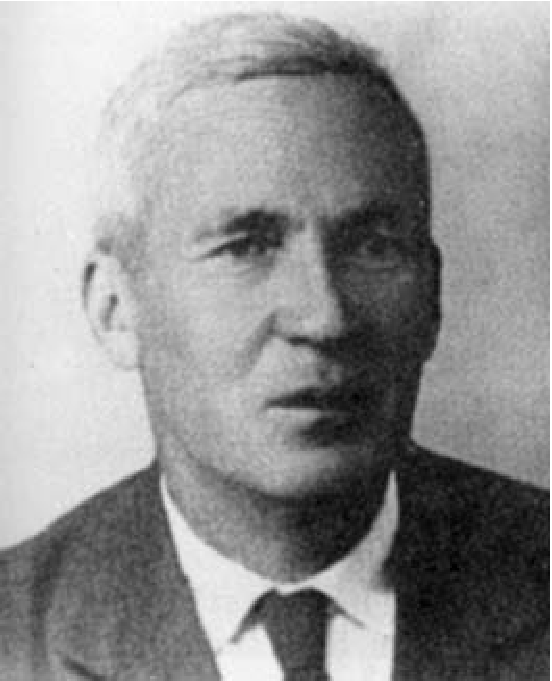
\includegraphics[scale=0.25]{figures/Kolmogorov_7.pdf}
\end{center}

\pause
\item The axiomatic approach is not concerned with the interpretation of probabilities.
\item Concerned only that probabilities are defined by a function satisfying the axioms.
\pause
\item Kolmogorov (1903-1987) was one of the greatest
mathematicians of the 20th century. This axiomatization was one of his ``trivial'' accomplishment.
\end{itemize}
\end{frame}


%%%%%%%%%%%%%%%%%%%%%%%%%%%%%%%%%%%%%%%%%%
%%%%%%%%%%%%%%%%%%%%%%%%%%%%%%%%%%%%%%%%%%
\begin{frame}\frametitle{Axioms of probability}

\vspace{-0.3cm}
\begin{defn}
Let $P$ be a function that assigns a nonnegative real number to each event $E$ of a sample space $S$.
We call $P$ a \hl{probability} if
\pause
\begin{enumerate}
\item Axiom 1: non-negative \[0 \leq P(E)  \leq 1\]
\vspace{-0.7cm}
\pause
\item Axiom 2: total one \[P(S) =  1\]
\vspace{-0.7cm}
\pause
\item Axiom 3: countable addition
\[P\left(\underset{i=1}{\overset{\infty}{\bigcup}} E_i\right) = \sum_{i=1}^\infty P(E_i) \text{,  if } E_i \cap E_j=\O \text{ for } i \neq j  \]
\end{enumerate}
\end{defn}
\pause
In particular, for $k$ {\bf disjoint} events $E_1, \ldots, E_k$,
\[P\left(\underset{i=1}{\overset{k}{\bigcup}} E_i\right) = \sum_{i=1}^k P(E_i)\]
\end{frame}

%%%%%%%%%%%%%%%%%%%%%%%%%%%%%%%%%%%%%%%%%%
%\begin{frame}\frametitle{Examples of probability}
%Based on the initial survey, for a randomly selected student from this class,
%\begin{itemize}
%\item $P(\text{female}) = 39\%$.
%\item $P(\text{math major}) = 42\%$.
%\item $P(\text{has a part time job}) = 42\%$.
%\item $P(\text{vegetarian}) = 3\%$.
%\end{itemize}
%
%\end{frame}

%%%%%%%%%%%%%%%%%%%%%%%%%%%%%%%%%%%%%%%%%%
\section{Some simple propositions}
%%%%%%%%%%%%%%%%%%%%%%%%%%%%%%%%%%%%%%%%%%
\begin{frame}\frametitle{Propositions}
\begin{dinglist}{\DingListSymbolA}
\item Complement Rule:
\[P(A^c) = 1-P(A)\]
\end{dinglist}
%\vspace{0.2cm}
Proof (hint: use Axiom 2 and Axiom 3)


\vspace{3cm}
\pause
\begin{itemize}
\item $ P(\O) = 0 $
\end{itemize}

\end{frame}

%%%%%%%%%%%%%%%%%%%%%%%%%%%%%%%%%%%%%%%%%%
\begin{frame}%\frametitle{Propositions}
\begin{dinglist}{\DingListSymbolA}
\item Difference Rule:
\[  P(B \cap A^c) = P(B)-P(A) \text{, if } A \subseteq B \]
\end{dinglist}
%\vspace{0.2cm}
Proof (hint: use Axiom 3)


\vspace{3cm}
\pause
\begin{itemize}
\item $ P(B) \geq P(A) \text{, if } A \subseteq B $
\end{itemize}
Proof (hint: use Axiom 1)

\end{frame}


%%%%%%%%%%%%%%%%%%%%%%%%%%%%%%%%%%%%%%%%%%
\begin{frame}%\frametitle{Propositions}
\begin{dinglist}{\DingListSymbolA}
\item Inclusion-Exclusion: two events $A, B$ (not necessarily disjoint)
  \[ P(A \cup B) = P(A) + P(B) - P(A \cap B) \]
\end{dinglist}
%\vspace{0.2cm}
Proof (hint: use Axiom 3 and Venn-diagram)



\end{frame}


%%%%%%%%%%%%%%%%%%%%%%%%%%%%%%%%%%%%%%%%%%
\begin{frame}\frametitle{Inclusion-Exclusion example}
\disc{Suppose that for a randomly selected student in a probability class,
\begin{itemize}
\item $P(\text{live Eastern Time Zone at home}) = 63\%$.
\item $P(\text{senior}) = 41\%$.
\item $P(\text{live Eastern Time Zone at home and senior}) = 31\%$.
\end{itemize}
Find the probability that a student is either live Eastern Time Zone at home or a senior.
}
\pause
\begin{enumerate}
\item \underline{Conditions}: event $A = \{\text{live Eastern Time Zone at home}\}$, $B = \{ \text{senior} \}$,
\[P(A) = 0.63, P(B) = 0.41, P(A \cap B) = 0.31\] \pause\vspace{-0.5cm}
\item \underline{Question}: find $P(A \cup B)$.\pause
\item \underline{Formula}: inclusion-exclusion
\[P(A \cup B) = P(A) + P(B) - P(A \cap B) = 0.63 + 0.41 - 0.31 = 0.73\]
\end{enumerate}


\end{frame}




%%%%%%%%%%%%%%%%%%%%%%%%%%%%%%%%%%%%%%%%%%
\begin{frame}\frametitle{Propositions}
\begin{dinglist}{\DingListSymbolA}
\item Inclusion-Exclusion: three events $A, B, C$ (not necessarily disjoint)
  \begin{align*}
  P(A \cup B \cup C) = & P(A) + P(B) + P(C) - P(A \cap B) \\
                  		  & - P(A \cap C)  - P(B \cap C) + P(A \cap B \cap C)
  \end{align*}
\end{dinglist}
\begin{center}
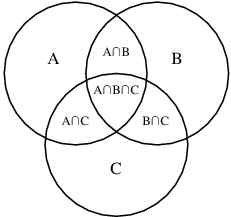
\includegraphics[width=0.45\textwidth]{Figures/venn.png}
\end{center}


\end{frame}


%%%%%%%%%%%%%%%%%%%%%%%%%%%%%%%%%%%%%%%%%%
\begin{frame}\frametitle{Recap}

Three axioms of probability $P$
\begin{enumerate}
\item $0 \leq P(E)  \leq 1$
\item $P(S) =  1$
\item $P\left(\underset{i=1}{\overset{\infty}{\cup}} E_i\right) = \sum_{i=1}^\infty P(E_i) \text{,  if } E_i \cap E_j=\emptyset \text{ for } i \neq j$
\end{enumerate}

\pause
Propositions of probability
\begin{itemize}
\item $P(A^c) = 1-P(A)$
\item $P(B \cap A^c) = P(B)-P(A) \text{, if } A \subseteq B$
\item $P(A \cup B) = P(A) + P(B) - P(A \cap B)$
\item $P(A \cup B \cup C) = P(A) + P(B) + P(C) - P(A \cap B) - P(A \cap C)  - P(B \cap C) + P(A \cap B \cap C)$
\end{itemize}


\end{frame}

%%%%%%%%%%%%%%%%%%%%%
%\begin{frame}{Outline}
%%\tableofcontents[hideallsubsections,pausections]
%\tableofcontents[hideallsubsections]
%\end{frame}




%%%%%%%%%%%%%%%%%%%%%%%%%%%%%%%%%%%%%%%%%%
\section{Sample spaces with equally likely outcomes}
%%%%%%%%%%%%%%%%%%%%%%%%%%%%%%%%%%%%%%%%%%
\begin{frame}\frametitle{Sample spaces with equally likely outcomes}
\begin{dinglist}{\DingListSymbolA}
\item Suppose a sample space has $N$ equally likely outcomes $\{1\}, \ldots, \{N\}$, then
\[
S = \{1\} \cup \ldots \cup \{N\}
\]
Disjointness gives
\[
1 = P(S) = P(\{1\}) + \ldots + P(\{N\}) = NP(\{i\}),
\]
so for each $1\leq i \leq N$,
\[
P(\{i\}) = \frac{1}{N}
\]

\uncover<2->{
\item For event $E$ in a sample space $S$ with equally likely outcomes,
\[P(E) = \frac{\#(E)}{\#(S)}  \] %=  \sum_i \frac{1_{ \omega_i \in E}}{\#(S)}\]

Notation: \\
\vspace{2mm} \hspace{2mm} Cardinality - $\#(E) =  \text{number of elements in set } E$\\
}
\end{dinglist}
\end{frame}


%%%%%%%%%%%%%%%%%%%%%%%%%%%%%%%%%%%%%%%%%%

\begin{frame}%\frametitle{TBD}
\vfill
\disc{Probability of rolling an even number with a six sided die?}
\pause
\[ E = \{2,4,6\} \text{ and } S = \{1,2,3,4,5,6\}\]
\[P(E) = 3/6 = 1/2\]

\pause
\disc{A couple has two kids, what is the probability that they are not both girls? }
\pause
\[ E = \{ BB, GB, BG \}  \text{ and } S = \{ BB, GG, GB, BG \} \]
\[P(E) = 3/4 \]


\end{frame}



%%%%%%%%%%%%%%%%%%%%%%%%%%%%%%%%%%%%%%%%%%

\begin{frame}[fragile]\frametitle{Example: birthday problem}

\disc{Ignoring leap years, and assuming birthdays are equally likely to be any day of the year,
what is the chance of no tie in birthdays among $n$ students?}

%\pause %\vspace{5mm}

%What would you guess the probability is?

\pause %\vspace{2mm}

\vspace{-4mm}
\begin{align*}
\#(\text{birthdays of $n$ people}) &= 365^n \\
\#(\text{no match}) &= 365 \times 364 \times \cdots \times (365 - n +1)\\
P(\text{no match}) &= \frac{365!}{(365-n)! ~365^n}
\end{align*}


\pause
\begin{center}
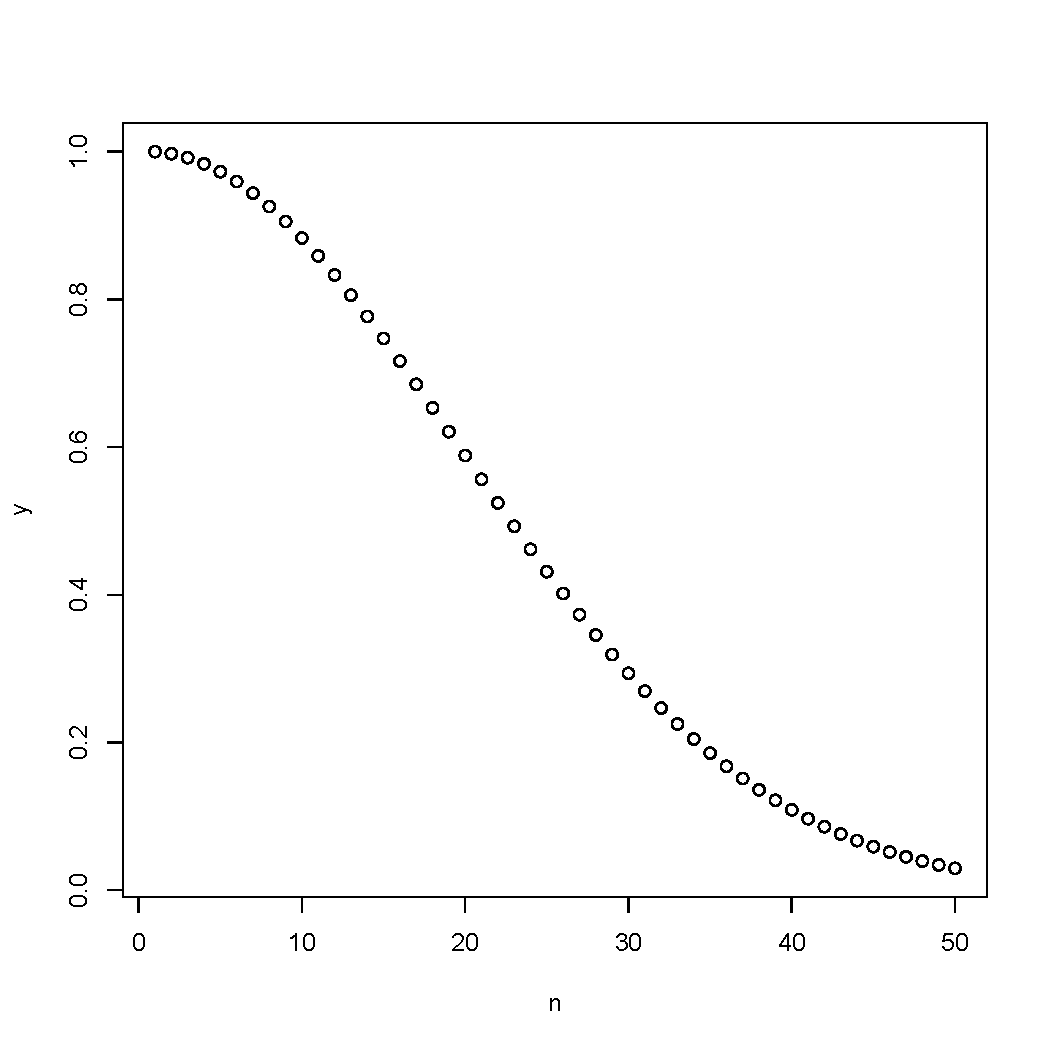
\includegraphics[width = 0.55\textwidth, height = 0.47\textheight]{figures/birthday}
\end{center}

\end{frame}


%%%%%%%%%%%%%%%%%%%%%%%%%%%%%%%%%%%%%%%%%%
%
%\begin{frame}
%\frametitle{$\log$ makes everything better}
%
%Remember:
%{\footnotesize
%\begin{align*}
%\log(XY) &= \log(X) + \log(Y)\\
%\log(X/Y) &= \log(X) - \log(Y)\\
%\log(X^b) &= b\log(X)
%\end{align*}
%}
%\pause
%\begin{itemize}
%\item Gamma function
%\[ \Gamma(n) = \int_0^\infty t^{n-1}e^{-t} dt\]
%\pause
%\item When $n$ is a positive integer,
%\[
%\Gamma(n+1) = n!
%\]
%\pause
%\item Most often a math library (include R) implement \texttt{gamma} and \texttt{lgamma}
%\end{itemize}
%
%\end{frame}
%

%%%%%%%%%%%%%%%%%%%%%%%%%%%%%%%%%%%%%%%%%%
%%%%%%%%%%%%%%%%%%%%%%%%%%%%%%%%%%%%%%%%%%%
%\begin{frame}%[fragile]\frametitle{ (5 cards)}
%\disc{Example: in a poker hand, what's the probability of getting one pair?}
%\pause
%Equally likely outcomes!
%\[
%P(\text{one pair}) = \frac{\#(\text{one pair among 5 cards})}{\#(\text{all possible combanions})}
%\]
%
%\pause
%\begin{center}
%\begin{tabular}{ccccc}
%\underline{\hspace{1cm}} & \underline{\hspace{1cm}} & \underline{\hspace{1cm}} & \underline{\hspace{1cm}} & \underline{\hspace{1cm}} \\
%a & a & b & c & d\\
%\end{tabular}
%\end{center}
%
%\pause
%Order doesn't matter! Count the number of combinations.
%
%\[\#(\text{one pair})  = {13 \choose 1}{4 \choose 2}{12 \choose 3}{4 \choose 1}{4 \choose 1}{4 \choose 1}\]
%\[\#(\text{poker hand})  = {52 \choose 5}\]
%
%
%\[
%P(\text{one pair})  = \frac{\#(\text{one pair}) }
%				 {\#(\text{poker hand})} = 0.42
%\]
%
%
%\end{frame}
%
%
%%%%%%%%%%%%%%%%%%%%%%%%%%%%%%%%%%%%%%%%%%%
%%\begin{frame}\frametitle{How many ways of getting one pair?}
%%
%%\begin{center}
%%\begin{tabular}{ccccc}
%%\underline{\hspace{1cm}} & \underline{\hspace{1cm}} & \underline{\hspace{1cm}} & \underline{\hspace{1cm}} & \underline{\hspace{1cm}} \\
%%a & a & b & c & d\\
%%\end{tabular}
%%\end{center}
%%
%%\[
%%\#(\text{one pair}) = {13 \choose 1}{4 \choose 2}{12 \choose 3}{4 \choose 1}{4 \choose 1}{4 \choose 1}
%%\]
%%
%%\pause
%%
%%Common mistakes
%%\vspace{0.3cm}
%%\begin{itemize}
%%\item
%%$\#(\text{one pair}) ={13 \choose 1}{12 \choose 3}$ \pause \hspace{1cm} \red{4 suits}
%%\pause
%%\item
%%$\#(\text{one pair}) ={13 \choose 1}{4 \choose 2} \times {12 \choose 1}{4 \choose 1}\times{11 \choose 1}{4 \choose 1}\times{10 \choose 1}{4 \choose 1}$\\
%%\pause  \red{The order among \{b, c, d\} does not matter.}
%%\item
%%$\#(\text{one pair}) ={13 \choose 4}{4 \choose 2}{4 \choose 1}{4 \choose 1}{4 \choose 1}$\\
%%\pause  \red{a is not exchangeable with b (or c or d).\\ \{aabcd\} and \{bbacd\} are different outcomes.}
%%
%%
%%\end{itemize}
%%
%%\end{frame}
%
%%%%%%%%%%%%%%%%%%%%%%%%%%%%%%%%%%%%%%%%%%%
%\begin{frame}[fragile]\frametitle{Poker hands (5 cards)}
%\disc{What's the probability of getting two pairs?}
%
%\begin{center}
%\begin{tabular}{ccccc}
%\underline{\hspace{1cm}} & \underline{\hspace{1cm}} & \underline{\hspace{1cm}} & \underline{\hspace{1cm}} & \underline{\hspace{1cm}} \\
%a & a & b & b & c\\
%\end{tabular}
%\end{center}
%
%\pause
%Order doesn't matter! Count the number of combinations.
%
%\[\#(\text{2 pairs})  = {13 \choose 2}{4 \choose 2}{4 \choose 2}{11 \choose 1}{4 \choose 1}\]
%\[\#(\text{poker hand})  = {52 \choose 5}\]
%
%
%\[
%P(\text{2 pairs})  = \frac{\#(\text{2 pairs}) }
%				 {\#(\text{poker hand})} = 0.048
%\]
%
%
%
%%\pause
%%\[
%%P(\text{2 pairs})  = \frac{{13 \choose 2}{4 \choose 2}{4 \choose 2}{11 \choose 1}{4 \choose 1}}
%%				 {{52 \choose 5}} = 0.047539
%%\]
%%
%%\pause
%%
%%\disc{What's the probability of getting 3 of a kind?}
%%
%%\begin{center}
%%\begin{tabular}{ccccc}
%%\underline{\hspace{1cm}} & \underline{\hspace{1cm}} & \underline{\hspace{1cm}} & \underline{\hspace{1cm}} & \underline{\hspace{1cm}} \\
%%a & a & a & b & c\\
%%\end{tabular}
%%\end{center}
%%
%%\pause
%%\[
%%P(\text{3 of a kind})  = \frac{{13 \choose 1}{4 \choose 3}{12 \choose 2}{4 \choose 1}{4 \choose 1}}
%%				 {{52 \choose 5}} = 0.021128
%%\]
%
%\end{frame}
%
%
%%%%%%%%%%%%%%%%%%%%%%%%%%%%%%%%%%%%%%%%%%%%
%%\begin{frame}[fragile]\frametitle{Poker hands (5 cards)}
%%\disc{What's the probability of getting a full house?}
%%
%%\begin{center}
%%\begin{tabular}{ccccc}
%%\underline{\hspace{1cm}} & \underline{\hspace{1cm}} & \underline{\hspace{1cm}} & \underline{\hspace{1cm}} & \underline{\hspace{1cm}} \\
%%a & a & a & b & b\\
%%\end{tabular}
%%\end{center}
%%
%%
%%\pause
%%\[
%%P(\text{full house})  = \frac{{13 \choose 1}{4 \choose 3}{12 \choose 1}{4 \choose 2}}
%%				 {{52 \choose 5}} = 0.0014
%%\]
%%
%%\pause
%%
%%\disc{What's the probability of getting a flush?}
%%
%%\begin{center}
%%\begin{tabular}{ccccc}
%%\underline{\hspace{1cm}} & \underline{\hspace{1cm}} & \underline{\hspace{1cm}} & \underline{\hspace{1cm}} & \underline{\hspace{1cm}} \\
%%\end{tabular}
%%\end{center}
%%\begin{center}
%%\begin{tabular}{c}
%%from the same suit
%%\end{tabular}
%%\end{center}
%%
%%\pause
%%\[
%%P(\text{flush})  = \frac{{13 \choose 5}{4 \choose 1}}
%%				 {{52 \choose 5}} = 0.001981
%%\]
%%
%%\end{frame}
%%
%
%
%%%%%%%%%%%%%%%%%%%%%%%%%%%%%%%%%%%%%%%%%%




%%%%%%%%%%%%%%%%%%%%%%%%%%%%%%%%%%%%%%%%%%



%%%%%%%%%%%%%%%%%%%%%%%%%%%%%%%%%%%%%%%%%%


\end{document}
